\section{Løsningsalgoritmer}

For at finde en $k$-approksimation, der løser et tilfælde af TSP, viser det sig, at problemet da nødvendigvis skal restringeres til eksempelvis den metriske version, jf. Korollar \ref{thm:korollar}.
Selvom der ikke findes nogen polynomiel løsning til TSP, er det dog stadig muligt at finde på en løsningsalgoritme.

Den mest umiddelbare løsningsalgoritme til at finde en kortest mulig Hamiltonkreds rundt i en graf, finder samtlige mulige Hamiltonkredse i grafen. Til hver af disse kredse beregnes den samlede vægt, og til sidst sammenlignes alle disse samlede vægte, for at finde den Hamiltonkreds, som har den mindste samlede vægt. Denne algoritme er i pseudokode beskrevet i Algoritme \ref{brute_force}.

\begin{algorithm}
\caption{Brute-force algoritmen}
\label{brute_force}
\textbf{procedure} Find korteste Hamiltonkreds i grafen $G$.

Bestem alle Hamiltonkredse, $H$, i $G$, og lad $H_{i}$ betegne den $i$'te Hamiltonkreds. \\
	$min := d(H_{1})$ \\
	$\alpha :=$ antallet af Hamiltonkredse \\
\textbf{for} $i:=2$ til $\alpha$ \\
$\-$ $\-$ $\-$ $\-$ $\-$ $\-$
	\textbf{hvis} $min > d(H_{i})$ \textbf{så} $min := d(H_{i})$ \\
\textbf{returnér} $min$ $\lbrace$ $min$ er længden af den korteste Hamiltonkreds i $G$ $\rbrace$
\end{algorithm}

Denne algoritme vil altid finde den kortest mulige Hamiltonkreds i en komplet graf $G$, men kræver meget tid at gennemføre, selv for grafer med relativt få knuder \citep{dmat}.

\begin{thm}
	Den værst mulige tidskompleksitet af Brute-force Algoritmen er $\Theta((n-1)!)$.
\end{thm}

\begin{proof}
	Lad $G$ være en komplet graf med $n$ knuder og $n \geq 3$.
	I denne graf er der så $(n-1)!$ forskellige Hamiltonkredse, idet de $n-1$ punkter kan arrangeres på $(n-1)!$ forskellige måder.
	Antallet af sammenligninger i Algoritme \ref{brute_force} er det samme som antallet af gentagelser i for-løkken.
	Dette er det samme om antallet af hamiltonkredse minus 1, og da må antallet af sammenligninger være $(n-1)! -1$.  	

	Det vises nu at $(n-1)! -1$ er $\Theta((n-1)!)$.

	Lad antallet af sammenligninger $f(n) = (n-1)! -1$, og lad $n > 2$.
	Da må $f(n)$ være $O((n-1)!)$, siden
	\begin{align*}
		(n-1)! -1 \leq (n-1)!
	\end{align*}
	når $n>2$. Da er vidnerne $k=2$ og $C=1$.
	
	Funktionen $f(n)$ må også være $\Omega((n-1)!)$, da
	\begin{align*}
		(n-1)! -1 \geq (n-1)! - \frac{(n-1)!}{2} = \frac{(n-1)!}{2}
	\end{align*}
	når $n>2$. Da er vidnerne $k=2$ og $C=\frac{1}{2}$.

	Eftersom $f(n)$ både er $O((n-1)!)$ og $\Omega((n-1)!)$ må $f(n)$ også være $\Theta((n-1)!)$. Da er tidskompleksiteten af Brute-force algortimen $\Theta((n-1)!)$.
\end{proof}

Brute-force algoritmen har således en kompleksitet, der er voldsom stor selv ved relativt få knuder i $G$.

\begin{exmp}
I den komplette graf, $G$, med $20$ knuder, foretager brute-force algoritmen $$19! = 121645100408832000,$$ sammenligninger, hvorfor algoritmen tydeligvis allerede ved $20$ knuder er håbløs, da det er svært at forestille sig en computer, der hurtigt kan udregne dette antal sammenligninger.
\end{exmp}

Derfor er approksimationsalgoritmer nødvendige, for at løse problemet. Som tidligere beskrevet, vil disse algoritmer \textit{ikke} finde den optimale løsning, men en løsning, som ligger indenfor en vis konstant grænse. I denne rapport vil Dobbelttræ-algoritmen anvendes til at løse TSP. 

\subsection{Dobbelttræ-algoritmen}
Dobbelttræ-algoritmen forudsætter, at grafen, som Hamiltonkredsen skal findes i, er komplet metrisk. For sådanne grafer kan der imidlertid foretages en \textit{genvej}, som defineres i Definition \ref{def_genvej}.

\begin{defn}
Lad $G$ være en komplet, metrisk graf med $n$ knuder og $n \geq 3$. Lad $P$ være en vej i $G$, $P = v_0, v_1,...,v_{i-1}, v_i, v_{i+1},...,v_{n-1},v_n$ hvor $1 \leq i \leq n-1$.

	Da kan der dannes en \textit{genvej} i $P$ via $e=\lbrace v_{i-1}, v_{i+1} \rbrace$, udenom $v_i$, så en ny vej, $P'=v_0, v_1,...,v_{i-1},v_{i+1},...,v_{n+1},v_n$, dannes. Her er $\lbrace v_i \rbrace = P \setminus P'$.
\label{def_genvej}
\end{defn}

Det gælder desuden for en genvej i en vej, $P$, udenom knuden $v_i$, hvor $v_{i-1}$ og $v_{i+1}$ var dets naboer i vejen, at den nye vej, $P'$ er kortere end den forrige, da grafen er metrisk og opfylder den trekantsuligheden.

\begin{tcolorbox}
\begin{lem}\label{lem:genvej}
Lad $P$ være en vej, og $P'$ en genvej i $P$ udenom $v_i$. Da følger det, at $P'$ er en kortere vej end $P$.
\end{lem}
\end{tcolorbox}

\begin{proof}
Lad $G$ være en komplet, metrisk graf. Da gælder trekantsuligheden for alle tripler af knuder i grafen, så $d(v_{i-1},v_{i+1}) \leq d(v_{i-1}, v_i) + d(v_i, v_{i+1})$. Da følger det, at $d(P') \leq d(P)$. 
\end{proof}

I en komplet, metrisk graf $G$ begynder Dobbelttræ-algoritmen med, at finde et minimalt udspændende træ, $T$, ved hjælp af Prims Algoritme.
Når $T$ er fundet, fordobles alle kanter i $T$, som så danner en multigraf $D$.
Graden af alle knuder i $D$ må være lige, hvorfor der må eksistere en Eulerkreds i $D$, jf. Sætning \ref{Eulerkreds_multigraf}.
Eulerkredsen dannes ved Algoritme \ref{algoritme_euler}.
I denne Eulerkreds skydes der genvej udenom en knude, hvis knuden allerede er med i kredsen, for at opnå en Hamiltonkreds, $H$.
Denne algoritme er sammenfattet i Algoritme \ref{dt_algo}.

\begin{algorithm}[h]
\caption{Dobbelttræ-algoritme}
\label{dt_algo}
\textbf{procedure} En metrisk komplet graf, $G$ \\
Find minimalt udspændende træ, $T$, i $G$ $\lbrace$ Algoritme \ref{find_mintrae} $\rbrace$. \\
$D := T$ \\
\textbf{for} kant \textbf{i} $D$ \\
$\-$ $\-$ $\-$ $\-$ $\-$ $\-$
dublér kant \\
Find Eulerkreds, $E$, i $D$ $\lbrace$ Algoritme \ref{algoritme_euler} $\rbrace$ \\
Skyd genvej i $E$ for at opnå Hamiltonkredsen, $H$ \\
\textbf{returnér} $H$ $\lbrace$ $H$ er Hamiltonkreds i $G$ $\rbrace$
\end{algorithm}

\begin{figure}[htbp]
\centering
	\begin{minipage}[t]{0.5\textwidth}
		\centering
			\scalebox{0.7}{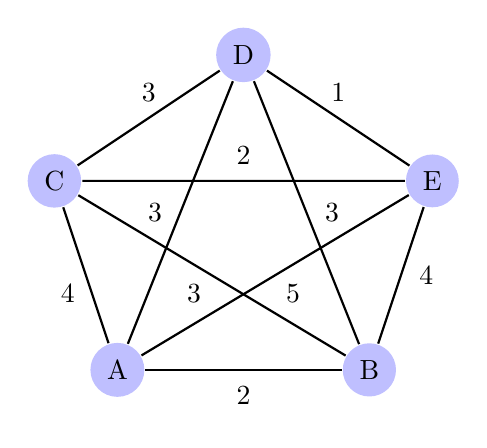
\begin{tikzpicture}
[thick,scale=.8,auto=left,every node/.style={circle,fill=blue!25}]
  \node (na) at (2,0) {A};
  \node (nb) at (6,0) {B};
  \node (nc) at (1,3) {C};
  \node (nd) at (4,5) {D};
  \node (ne) at (7,3) {E};
  \path[-,draw,thick,black]
  	(na) edge node[draw=none,fill=none,below] {$2$} (nb)
  	(nb) edge node[draw=none,fill=none,right] {$4$} (ne)
  	(ne) edge node[draw=none,fill=none,above] {$1$} (nd)
  	(nd) edge node[draw=none,fill=none,above] {$3$} (nc)
  	(nc) edge node[draw=none,fill=none,below left] {$3$} (nb)
  	(na) edge node[draw=none,fill=none] {$4$} (nc)
  	(na) edge node[draw=none,fill=none,below right] {$5$} (ne)
  	(na) edge node[draw=none,fill=none,left] {$3$} (nd)
  	(nd) edge node[draw=none,fill=none,right] {$3$} (nb)
  	(nc) edge node[draw=none,fill=none] {$2$} (ne);
\end{tikzpicture}

  %\path[-,draw,black]
  	%(n3) edge node[draw=none,fill=none] {$e$} (n7);
  %\path[-,draw,very thick,blue,bend right]
  	%(n6) edge node[draw=none,fill=none,color=black] {$e'$} (n7);
  	
  	
 	%\node (n6) at (2,0) {A};
  %\node (n4) at (6,0) {B};
  %\node (n5) at (0,4) {C};
  %\node (n1) at (4,6) {D};
  %\node (n2) at (8,4) {E};
  %\foreach \from/\to in {n6/n5,n4/n2}
    %\draw (\from) -- (\to);}
		\label{dtex1}
		\subcaption[first caption.]{Komplet vægtet metrisk graf med 5 knuder.}\label{fig:1a}
	\end{minipage}%
	\begin{minipage}[t]{0.5\textwidth}
		\centering
			\scalebox{0.7}{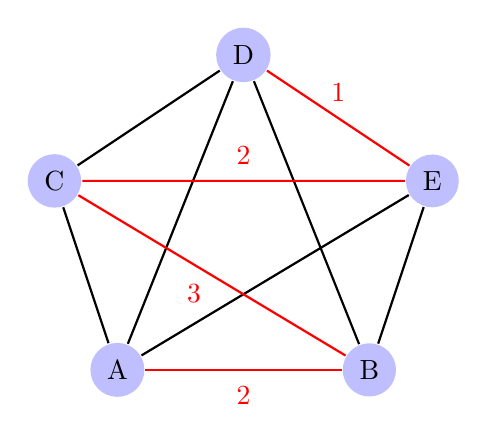
\begin{tikzpicture}
[thick,scale=.8,auto=left,every node/.style={circle,fill=blue!25}]
  \node (na) at (2,0) {A};
  \node (nb) at (6,0) {B};
  \node (nc) at (1,3) {C};
  \node (nd) at (4,5) {D};
  \node (ne) at (7,3) {E};
  \path[-,draw,thick,black]
  	(ne) edge (nb)
  	(nd) edge (nc)
  	(na) edge (nc)
  	(na) edge (ne)
  	(na) edge (nd)
  	(nd) edge (nb);
  	
  \path[-,draw,thick,red]
  	(na) edge node[draw=none,fill=none,below] {$2$} (nb)
  	(nc) edge node[draw=none,fill=none,below left] {$3$} (nb)
  	(nc) edge node[draw=none,fill=none] {$2$} (ne)
  	(ne) edge node[draw=none,fill=none,above] {$1$} (nd);
\end{tikzpicture}}
		\label{dtex2}
		\subcaption[second caption.]{Minimalt undspændende træ findes i grafen.}\label{fig:1b}
	\end{minipage}

	\vspace{10mm}

	\begin{minipage}[t]{0.5\textwidth}
		\centering		
			\scalebox{0.7}{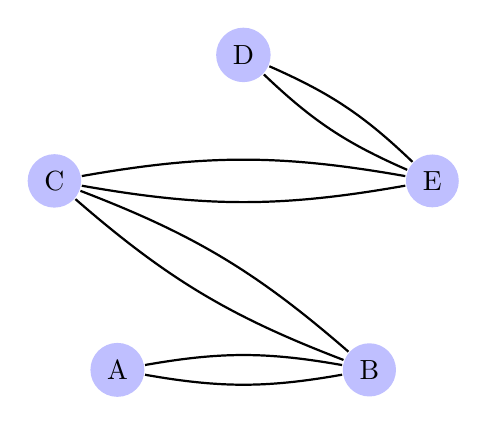
\begin{tikzpicture}
[thick,scale=.8,auto=left,every node/.style={circle,fill=blue!25}]
  \node (na) at (2,0) {A};
  \node (nb) at (6,0) {B};
  \node (nc) at (1,3) {C};
  \node (nd) at (4,5) {D};
  \node (ne) at (7,3) {E};

  \path[-,draw,thick,black,bend right=10]
  	(na) edge (nb)
  	(nc) edge (nb)
  	(nc) edge (ne)
  	(ne) edge (nd);
  
  \path[-,draw,thick,black,bend left=10]
  	(na) edge (nb)
  	(nc) edge (nb)
  	(nc) edge (ne)
  	(ne) edge (nd);
\end{tikzpicture}}
		\label{dtex3}
		\subcaption[third caption.]{Alle kanter i træet fordobles.}\label{fig:1c}
	\end{minipage}%
	\begin{minipage}[t]{0.5\textwidth}
		\centering
			\scalebox{0.7}{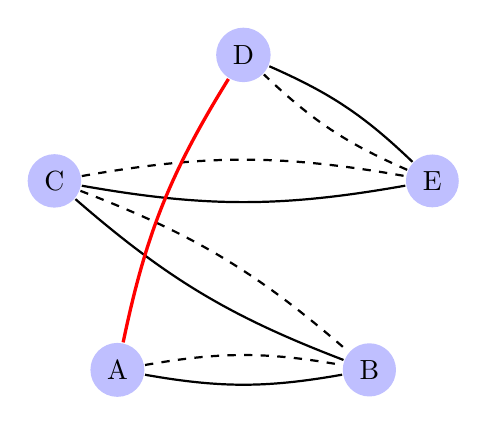
\begin{tikzpicture}
[thick,scale=.8,auto=left,every node/.style={circle,fill=blue!25}]
  \node (na) at (2,0) {A};
  \node (nb) at (6,0) {B};
  \node (nc) at (1,3) {C};
  \node (nd) at (4,5) {D};
  \node (ne) at (7,3) {E};

  \path[-,draw,thick,black,bend right=10]
  	(na) edge (nb)
  	(nc) edge (nb)
  	(nc) edge (ne)
  	(ne) edge (nd);
  
  \path[dashed,draw,thick,black,bend left=10]
  	(na) edge (nb)
  	(nc) edge (nb)
  	(nc) edge (ne)
  	(ne) edge (nd);
  	
  \path[-,draw,very thick,red,bend right=10]
  	(nd) edge (na);
  	
\end{tikzpicture}}
		\label{dtex4}
		\subcaption[fourth caption.]{Der skydes genvej i Eulerkredsen for at danne en Hamiltonkreds.}\label{fig:1d}
	\end{minipage}

	\vspace{5mm}

	\caption{} \label{fig:1}
\end{figure}

\begin{exmp}
	Som eksempel på Dobbelttræ-Algoritmens fremgangsmåde, ses på en komplet, metrisk graf med $5$ knuder.
På Figur \ref{fig:1a} ses grafen, som der nu skal findes en Hamiltonkreds i.
	Algoritmen finder så et minimalt udspændende træ ved Prims algoritme som i Figur \ref{fig:1b}.
	Herefter ses bort fra de resterende kanter, som ikke er en del af træet, og samtlige kanter i det minimalt udspændende træ fordobles, som det er gjort i Figur \ref{fig:1c}.
	Slutteligt skydes der flere genveje, som på Figur \ref{fig:1d} ses som den røde kant, som indsættes til fordel for de stiplede kanter. Dermed er der fundet en Hamiltonkreds.
\end{exmp}

\subsection{Kompleksitet af Dobbelttræ-algoritmen}
Dobbelttræ-algoritmen er en approksimationsalgoritme, som det er bevist ovenfor. Derfor må det formodes, at den har en lavere kompleksitet end Brute-force Algoritmen havde.

\begin{thm}
Dobbelttræ-algoritmen har en værst mulig tidskompleksitet på $O(n^3)$.
\end{thm}

\begin{proof}
Dobbelttræ-algoritmen kører først Prims Algoritme, som er $O(n^3)$, jf. Sætning \ref{prim_kompl}. 
Herefter er antallet af kanter $|E|=n-1$.
Derefter fordobler algoritmen samtlige kanter i træet, som Prims Algoritme har dannet, og da er antallet af kanter $|E|=2(n-1)$.
	Denne tilfører kompleksiteten $O(n)$.
	Så kører Dobbelttræ-algoritmen algoritmen for dannelsen af en Eulerkreds, som har lineær værst mulig tidskompleksitet, altså også $O(|E|)$ jf. Sætning \ref{thm:O_euler}. 
Siden $2(n-1)$ er $O(n)$ må denne del af Dobbelttræ-algoritmen også have en lineær tidskompleksitet.
Slutteligt vil Dobbelttræ-algoritmen skyde genvej hver gang den møder en knude der allerede er med i kredsen, og da danne en Hamiltonkreds. Antallet af sammenligninger der skal foretages for ved hver knude at beslutte om der skal skydes en genvej, må være det samme antal som der er kanter i det fordoblede træ, altså $2(n-1)$.
	Da må denne del af algoritmen have tidskompleksiteten $O(n)$.

	Derfor må den værst mulige tidskompleksitet af Dobbelttræ-algoritmen være $O(n^3)$.
\end{proof}

Dobbelttræ-algoritmen viser sig altså at være af polynomiel værst mulig tidskompleksitet, hvorfor denne noget hurtigere vil finde en kort Hamiltonkreds i grafen. Dog er det på det kompromis, at det ikke nødvendigvis er den korteste Hamiltonkreds i $G$.

\begin{exmp}
I den komplette graf, $G$, med $20$ knuder, har Dobbelttræ-algoritmen en værst mulig tidskompleksitet på $O(n^3)$ og må da foretager $$20^3 = 8000$$ sammenligninger. Den er derfor markant hurtigere end Brute-force Algoritmen.
\end{exmp}

\subsection{Præcision af Dobbelttræ-algoritmen}
Dobbelttræ-algoritmen finder en Hamiltonkreds som er en approksimation af den optimale løsning til det metriske TSP.

\begin{thm}
Dobbelttræ-algoritmen er en 2-approksimation.
\end{thm}

\begin{proof}
Lad $H$ være Hamiltonkredsen af lavest muligt vægt i grafen $G$ og $H'$ være den Hamiltonkreds, som Dobbelttræ-algoritmen finder ved genvej i Eulerkredsen $E$. Der må ifølge Lemma \ref{lem:genvej} gælde, at 
\begin{align*}
	d(H')\leq d(E).
\end{align*}
Idet Eulerkredsen, $E$, er dannet ved at dublere alle kanter i det minimalt udspændende træ, $T$, må der gælde, at 
\begin{align*}
	d(E) = 2d(T).
\end{align*}
Eftersom enhver Hamiltonkreds ved fjernelse af en kant danner et udspændende træ, må der gælde, at $d(T) \leq d(H)$.
	Heraf følger det, at
	\begin{align*}
		2d(T) \leq 2d(H').
	\end{align*}
Derfor må der gælde, at 
	\begin{align*}
		d(H') \leq 2d(H).
	\end{align*}
	Fordi kompleksiteten af Dobbelttræ-algoritmen er polynomiel, kan det siges, at den er en $2$-approksimation. 
\end{proof}
